%% uncomment to list all files in log
%\listfiles

\documentclass[12pt]{report}


\usepackage{fontspec}

%\setmainfont[Scale=MatchLowercase]{Lucida Bright}
%\setmonofont{FreeMono}
%\setmonofont{Source Code Pro}
\setmonofont[Scale=MatchLowercase]{Ubuntu Mono}

\usepackage[headings]{fullpage}

% national use characters 
%\usepackage{inputenc}

% ams mathematical symbols
\usepackage{amsmath,amssymb}

% added to support pandoc highlighting
\usepackage{microtype}

\usepackage{makeidx}

% add index and bibliographies to table of contents
\usepackage[nottoc]{tocbibind}

% postscript courier and times in place of cm fonts
%\usepackage{courier}
%\usepackage{times}

% extended coloring
\usepackage{color}
\usepackage[table,dvipsnames]{xcolor}
\usepackage{colortbl}

% advanced date formating
\usepackage{datetime}

%support pandoc code highlighting
\usepackage{fancyvrb}
\DefineShortVerb[commandchars=\\\{\}]{\|}
\DefineVerbatimEnvironment{Highlighting}{Verbatim}{commandchars=\\\{\}}
% Add ',fontsize=\small' for more characters per line

%tango style colors
% \usepackage{framed}
% \definecolor{shadecolor}{RGB}{255,255,255}
% \newenvironment{Shaded}{\begin{snugshade}}{\end{snugshade}}
% \newcommand{\KeywordTok}[1]{\textcolor[rgb]{0.13,0.29,0.53}{\textbf{{#1}}}}
% \newcommand{\DataTypeTok}[1]{\textcolor[rgb]{0.13,0.29,0.53}{{#1}}}
% \newcommand{\DecValTok}[1]{\textcolor[rgb]{0.00,0.00,0.81}{{#1}}}
% \newcommand{\BaseNTok}[1]{\textcolor[rgb]{0.00,0.00,0.81}{{#1}}}
% \newcommand{\FloatTok}[1]{\textcolor[rgb]{0.00,0.00,0.81}{{#1}}}
% \newcommand{\CharTok}[1]{\textcolor[rgb]{0.31,0.60,0.02}{{#1}}}
% \newcommand{\StringTok}[1]{\textcolor[rgb]{0.31,0.60,0.02}{{#1}}}
% \newcommand{\CommentTok}[1]{\textcolor[rgb]{0.56,0.35,0.01}{\textit{{#1}}}}
% \newcommand{\OtherTok}[1]{\textcolor[rgb]{0.56,0.35,0.01}{{#1}}}
% \newcommand{\AlertTok}[1]{\textcolor[rgb]{0.94,0.16,0.16}{{#1}}}
% \newcommand{\FunctionTok}[1]{\textcolor[rgb]{0.00,0.00,0.00}{{#1}}}
% \newcommand{\RegionMarkerTok}[1]{{#1}}
% \newcommand{\ErrorTok}[1]{\textbf{{#1}}}
% \newcommand{\NormalTok}[1]{{#1}}

%espresso style colors
% \usepackage{framed}
% \definecolor{shadecolor}{RGB}{42,33,28}
% \newenvironment{Shaded}{\begin{snugshade}}{\end{snugshade}}
% \newcommand{\KeywordTok}[1]{\textcolor[rgb]{0.26,0.66,0.93}{\textbf{{#1}}}}
% \newcommand{\DataTypeTok}[1]{\textcolor[rgb]{0.74,0.68,0.62}{\underline{{#1}}}}
% \newcommand{\DecValTok}[1]{\textcolor[rgb]{0.27,0.67,0.26}{{#1}}}
% \newcommand{\BaseNTok}[1]{\textcolor[rgb]{0.27,0.67,0.26}{{#1}}}
% \newcommand{\FloatTok}[1]{\textcolor[rgb]{0.27,0.67,0.26}{{#1}}}
% \newcommand{\CharTok}[1]{\textcolor[rgb]{0.02,0.61,0.04}{{#1}}}
% \newcommand{\StringTok}[1]{\textcolor[rgb]{0.02,0.61,0.04}{{#1}}}
% \newcommand{\CommentTok}[1]{\textcolor[rgb]{0.00,0.40,1.00}{\textit{{#1}}}}
% \newcommand{\OtherTok}[1]{\textcolor[rgb]{0.74,0.68,0.62}{{#1}}}
% \newcommand{\AlertTok}[1]{\textcolor[rgb]{1.00,1.00,0.00}{{#1}}}
% \newcommand{\FunctionTok}[1]{\textcolor[rgb]{1.00,0.58,0.35}{\textbf{{#1}}}}
% \newcommand{\RegionMarkerTok}[1]{\textcolor[rgb]{0.74,0.68,0.62}{{#1}}}
% \newcommand{\ErrorTok}[1]{\textcolor[rgb]{0.74,0.68,0.62}{\textbf{{#1}}}}
% \newcommand{\NormalTok}[1]{\textcolor[rgb]{0.74,0.68,0.62}{{#1}}}

%kete style colors
% \newenvironment{Shaded}{}{}
% \newcommand{\KeywordTok}[1]{\textbf{{#1}}}
% \newcommand{\DataTypeTok}[1]{\textcolor[rgb]{0.50,0.00,0.00}{{#1}}}
% \newcommand{\DecValTok}[1]{\textcolor[rgb]{0.00,0.00,1.00}{{#1}}}
% \newcommand{\BaseNTok}[1]{\textcolor[rgb]{0.00,0.00,1.00}{{#1}}}
% \newcommand{\FloatTok}[1]{\textcolor[rgb]{0.50,0.00,0.50}{{#1}}}
% \newcommand{\CharTok}[1]{\textcolor[rgb]{1.00,0.00,1.00}{{#1}}}
% \newcommand{\StringTok}[1]{\textcolor[rgb]{0.87,0.00,0.00}{{#1}}}
% \newcommand{\CommentTok}[1]{\textcolor[rgb]{0.50,0.50,0.50}{\textit{{#1}}}}
% \newcommand{\OtherTok}[1]{{#1}}
% \newcommand{\AlertTok}[1]{\textcolor[rgb]{0.00,1.00,0.00}{\textbf{{#1}}}}
% \newcommand{\FunctionTok}[1]{\textcolor[rgb]{0.00,0.00,0.50}{{#1}}}
% \newcommand{\RegionMarkerTok}[1]{{#1}}
% \newcommand{\ErrorTok}[1]{\textcolor[rgb]{1.00,0.00,0.00}{\textbf{{#1}}}}
% \newcommand{\NormalTok}[1]{{#1}}
%end pandoc code hacks

% jodliterate colors
\usepackage{color}
\definecolor{shadecolor}{RGB}{248,248,248}
% j control structures 
\definecolor{keywcolor}{rgb}{0.13,0.29,0.53}
% j explicit arguments x y m n u v
\definecolor{datacolor}{rgb}{0.13,0.29,0.53}
% j numbers - all types see j.xml
\definecolor{decvcolor}{rgb}{0.00,0.00,0.81}
\definecolor{basencolor}{rgb}{0.00,0.00,0.81}
\definecolor{floatcolor}{rgb}{0.00,0.00,0.81}
% j local assignments
\definecolor{charcolor}{rgb}{0.31,0.60,0.02}
\definecolor{stringcolor}{rgb}{0.31,0.60,0.02}
\definecolor{commentcolor}{rgb}{0.56,0.35,0.01}
% primitive adverbs and conjunctions
%\definecolor{othercolor}{rgb}{0.56,0.35,0.01}   
\definecolor{othercolor}{RGB}{0,0,255}
% global assignments
\definecolor{alertcolor}{rgb}{0.94,0.16,0.16}
% primitive J verbs and noun names
\definecolor{funccolor}{rgb}{0.00,0.00,0.00}    

\usepackage{framed}
\newenvironment{Shaded}{}{}
\newcommand{\KeywordTok}[1]{\textcolor{keywcolor}{\textbf{{#1}}}}
\newcommand{\DataTypeTok}[1]{\textcolor{datacolor}{{#1}}}
%\newcommand{\DecValTok}[1]{\textcolor{decvcolor}{{#1}}}
\newcommand{\DecValTok}[1]{{#1}} 
\newcommand{\BaseNTok}[1]{\textcolor{basencolor}{{#1}}}
\newcommand{\FloatTok}[1]{\textcolor{floatcolor}{{#1}}}
\newcommand{\CharTok}[1]{\textcolor{charcolor}{\textbf{{#1}}}}
\newcommand{\StringTok}[1]{\textcolor{stringcolor}{{#1}}}
\newcommand{\CommentTok}[1]{\textcolor{commentcolor}{\textit{{#1}}}}
\newcommand{\OtherTok}[1]{\textcolor{othercolor}{{#1}}} 
\newcommand{\AlertTok}[1]{\textcolor{alertcolor}{\textbf{{#1}}}}
%\newcommand{\FunctionTok}[1]{\textcolor{funccolor}{{#1}}}
\newcommand{\FunctionTok}[1]{{#1}}
\newcommand{\RegionMarkerTok}[1]{{#1}}
\newcommand{\ErrorTok}[1]{\textbf{{#1}}}
\newcommand{\NormalTok}[1]{{#1}}

% headers and footers
\usepackage{fancyhdr}
\pagestyle{fancy}

\fancyhead{}
\fancyfoot{}

%\fancyhead[LE,RO]{\slshape \rightmark}
%\fancyhead[LO,RE]{\slshape \leftmark}
\fancyfoot[C]{\thepage}
%\headrulewidth 0.4pt
%\footrulewidth 0 pt

%\addtolength{\headheight}{\baselineskip}

%\lfoot{\emph{Analyze the Data not the Drivel}}
%\rfoot{\emph{\today}}

% subfigure handles figures that contain subfigures
%\usepackage{color,graphicx,subfigure,sidecap}
\usepackage{graphicx,sidecap}
\usepackage{subfigure}
\graphicspath{{./inclusions/}}

% floatflt provides for text wrapping around small figures and tables
\usepackage{floatflt}

% tweak caption formats 
\usepackage{caption} 
\usepackage{sidecap}
%\usepackage{subcaption} % not compatible with subfigure

\usepackage{rotating} % flip tables sideways

% complex footnotes
%\usepackage{bigfoot}

% weird logos \XeLaTeX
\usepackage{metalogo}

% source code listings
\usepackage{listings}

% long tables
% \usepackage{longtable}

\newcommand{\HRule}{\rule{\linewidth}{0.5mm}}

% map LaTeX cross references into PDF cross references
\usepackage[
            %dvips,
            colorlinks,
            linkcolor=blue,
            citecolor=blue,
            urlcolor=blue,   % magenta, cyan default        
            pdfauthor={John D. Baker},
            pdftitle={Analyze the Data not the Drivel},
            pdfsubject={Blog},
            pdfcreator={MikTeX+LaTeXe with hyperref package},
            pdfkeywords={blog,wordpress},
            ]{hyperref}
           
% custom colors
\definecolor{CodeBackGround}{cmyk}{0.0,0.0,0,0.05}    % light gray
\definecolor{CodeComment}{rgb}{0,0.50,0.00}           % dark green {0,0.45,0.08}
\definecolor{TableStripes}{gray}{0.9}                 % odd/even background in tables

\lstdefinelanguage{bat}
{morekeywords={echo,title,pushd,popd,setlocal,endlocal,off,if,not,exist,set,goto,pause},
sensitive=True,
morecomment=[l]{rem}
}

\lstdefinelanguage{jdoc}
{
morekeywords={},
otherkeywords={assert.,break.,continue.,for.,do.,if.,else.,elseif.,return.,select.,end.
,while.,whilst.,throw.,catch.,catchd.,catcht.,try.,case.,fcase.},
sensitive=True,
morecomment=[l]{NB.},
morestring=[b]',
morestring=[d]',
}

% latex size ordering - can never remember it
% \tiny
% \scriptsize
% \footnotesize
% \small
% \normalsize
% \large
% \Large
% \LARGE
% \huge
% \Huge
 
% listings package settings  
\lstset{%
  language=jdoc,                                % j document settings
  basicstyle=\ttfamily\footnotesize,            
  keywordstyle=\bfseries\color{keywcolor}\footnotesize,
  identifierstyle=\color{black},
  commentstyle=\slshape\color{CodeComment},     % colored slanted comments
  stringstyle=\color{red}\ttfamily,
  showstringspaces=false,                       
  %backgroundcolor=\color{CodeBackGround},       
  frame=single,                                
  framesep=1pt,                                 
  framerule=0.8pt,                             
  rulecolor=\color{CodeBackGround},   
  showspaces=false,
  %columns=fullflexible,
  %numbers=left,
  %numberstyle=\footnotesize,
  %numbersep=9pt,
  tabsize=2,
  showtabs=false,
  captionpos=b
  breaklines=true,                              
  breakindent=5pt                              
}

\lstdefinelanguage{JavaScript}{
  keywords={typeof, new, true, false, catch, function, return, null, catch, switch, var, if, in, while, do, else, case, break},
  ndkeywords={class, export, boolean, throw, implements, import, this},
  ndkeywordstyle=\color{darkgray}\bfseries,
  sensitive=false,
  comment=[l]{//},
  morecomment=[s]{/*}{*/},
  morestring=[b]',
  morestring=[b]"
}

% C# settings
\lstdefinestyle{sharpc}{
language=[Sharp]C,
basicstyle=\ttfamily\scriptsize, 
keywordstyle=\bfseries\color{keywcolor}\scriptsize,
framerule=0pt
}

% for source code listing longer than two use smaller font
\lstdefinestyle{smallersource}{
basicstyle=\ttfamily\scriptsize, 
keywordstyle=\bfseries\color{keywcolor}\scriptsize,
framerule=0pt
}

\lstdefinestyle{resetdefaults}{
language=jdoc,
basicstyle=\ttfamily\footnotesize,  
keywordstyle=\bfseries\color{keywcolor}\footnotesize,                                                               
framerule=0.8pt 
}

% APL UTF8 code points listed for lstlisting processing
\makeatletter
\lst@InputCatcodes
\def\lst@DefEC{%
 \lst@CCECUse \lst@ProcessLetter
  ^^80^^81^^82^^83^^84^^85^^86^^87^^88^^89^^8a^^8b^^8c^^8d^^8e^^8f%
  ^^90^^91^^92^^93^^94^^95^^96^^97^^98^^99^^9a^^9b^^9c^^9d^^9e^^9f%
  ^^a0^^a1^^a2^^a3^^a4^^a5^^a6^^a7^^a8^^a9^^aa^^ab^^ac^^ad^^ae^^af%
  ^^b0^^b1^^b2^^b3^^b4^^b5^^b6^^b7^^b8^^b9^^ba^^bb^^bc^^bd^^be^^bf%
  ^^c0^^c1^^c2^^c3^^c4^^c5^^c6^^c7^^c8^^c9^^ca^^cb^^cc^^cd^^ce^^cf%
  ^^d0^^d1^^d2^^d3^^d4^^d5^^d6^^d7^^d8^^d9^^da^^db^^dc^^dd^^de^^df%
  ^^e0^^e1^^e2^^e3^^e4^^e5^^e6^^e7^^e8^^e9^^ea^^eb^^ec^^ed^^ee^^ef%
  ^^f0^^f1^^f2^^f3^^f4^^f5^^f6^^f7^^f8^^f9^^fa^^fb^^fc^^fd^^fe^^ff%
  ^^^^20ac^^^^0153^^^^0152%
  ^^^^20a7^^^^2190^^^^2191^^^^2192^^^^2193^^^^2206^^^^2207^^^^220a%
  ^^^^2218^^^^2228^^^^2229^^^^222a^^^^2235^^^^223c^^^^2260^^^^2261%
  ^^^^2262^^^^2264^^^^2265^^^^2282^^^^2283^^^^2296^^^^22a2^^^^22a3%
  ^^^^22a4^^^^22a5^^^^22c4^^^^2308^^^^230a^^^^2336^^^^2337^^^^2339%
  ^^^^233b^^^^233d^^^^233f^^^^2340^^^^2342^^^^2347^^^^2348^^^^2349%
  ^^^^234b^^^^234e^^^^2350^^^^2352^^^^2355^^^^2357^^^^2359^^^^235d%
  ^^^^235e^^^^235f^^^^2361^^^^2362^^^^2363^^^^2364^^^^2365^^^^2368%
  ^^^^236a^^^^236b^^^^236c^^^^2371^^^^2372^^^^2373^^^^2374^^^^2375%
  ^^^^2377^^^^2378^^^^237a^^^^2395^^^^25af^^^^25ca^^^^25cb%  
  ^^00}
\lst@RestoreCatcodes
\makeatother

% custom lengths used within minipages
\newcommand{\minindent}{17pt}


\makeindex

\begin{document}

\subsection*{\href{http://bakerjd99.wordpress.com/2012/11/25/jhs-meets-mathjax/}{JHS meets MathJax}}
\addcontentsline{toc}{subsection}{JHS meets MathJax}


\noindent\emph{Posted: 25 Nov 2012 07:19:21}
\vspace{6pt}

\captionsetup[floatingfigure]{labelformat=empty}
\begin{floatingfigure}[r]{0.40\textwidth}
\centering
\href{http://bakerjd99.files.wordpress.com/2012/11/mathjaxdemo.png}{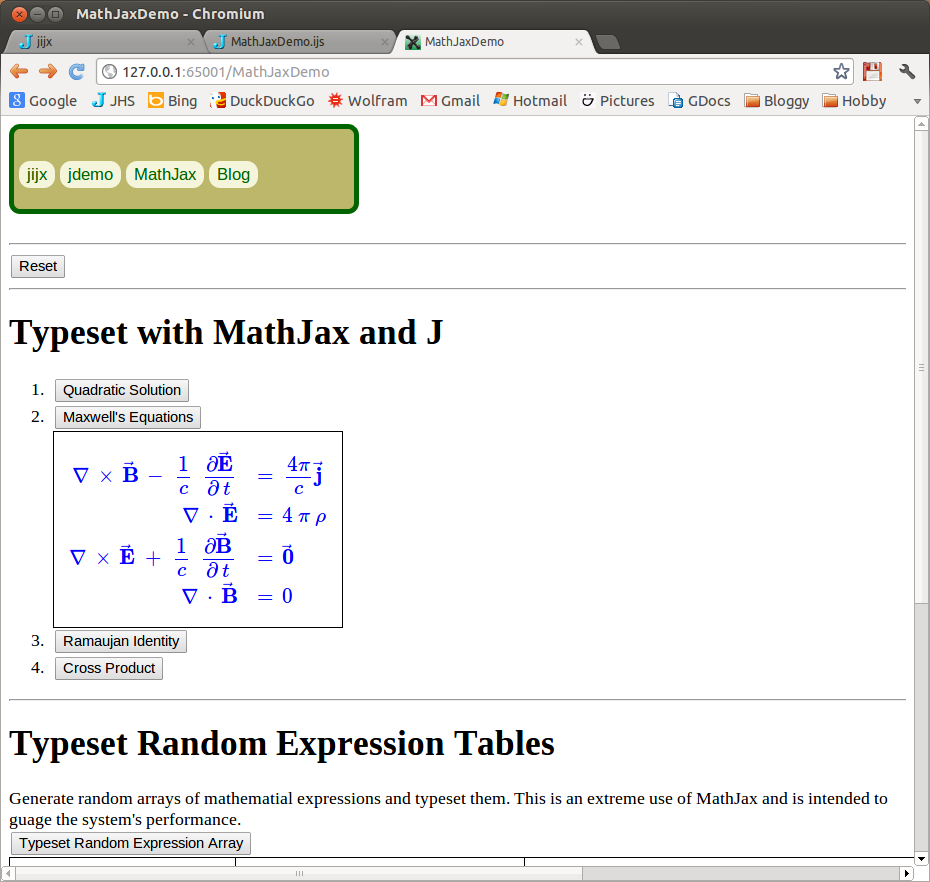
\includegraphics[width=0.37\textwidth]{mathjaxdemo.png}}
\caption{Screen shot of JHS MathJaxDemo running on Ubuntu}
\label{fig:3402X0}
\end{floatingfigure} With the release of J 7.01 \href{http://www.jsoftware.com}{Jsoftware}
``deprecated'' COM. J 6.02 can run as a
\href{http://en.wikipedia.org/wiki/OLE\_Automation}{COM automation server} 
but J 7.01 cannot. Throwing COM
\href{http://www.youtube.com/watch?v=aix35ZSp46c}{under the bus} is
hardly radical. Microsoft, COM's creator, has been holding COM's head
underwater for years. Many \texttt{.Net} programmers cringe when they
hear the word ``COM'' and the greater
nonwindows\footnote{
On a purely numerical basis there is no greater nonwindows world.
} world never \emph{really}
accepted it. COM is a complex, over-engineered, proprietary dead-end.
Yet despite its bloated deficiencies a lot of useful software is COM
based. So with COM going away, at least for J programmers, the hunt is
on for viable replacements and while we're hunting let's rethink our
entire approach to building J GUI applications.

J GUI applications are traditional desktop applications. They're built
on native GUIs like
\href{http://msdn.microsoft.com/en-us/library/dd30h2yb.aspx}{Windows
Forms} and \href{http://www.gtk.org/}{GTK} and when done well they look
and act like GUI applications coded in other languages. This is all good
but there is a fundamental problem with desktop GUIs. \emph{There are
many desktop GUIs and they do not travel well.} Programmers have spent
many dollars and days creating so-called \emph{cross-platform GUIs} but,
if you wander off the Windows, Mac and Linux reservation, the results
are not particularly portable. And, as portable GUIs rarely outperform
native alternatives, programmers tend to stick in their tribal silos.
GUI programming is a bitch, has always been a bitch and will always be a
bitch. It's time to divorce the desktop GUI bitch.

All divorces, even the geeky GUI variety, are hard. When you finally cut
the knot you're not entirely sure what you're doing or where you'll end
up. All you know is that there is a better way and with respect to J GUI
applications I believe that
\href{http://www.jsoftware.com/jwiki/NYCJUG/2011-02-08/HelloWorldInJHS}{JHS}
is that way. JHS leverages the large CSS, HTML and JavaScript (CHJ)
world and in recent years some impressive browser-based applications
have emerged from that world. The application that changed my mind about
JavaScript and browser-based applications in general is something called
\href{http://www.mathjax.org/}{MathJax}.

MathJax typesets mathematics. It renders both \LaTeX\ and MathML using
fully scalable browser fonts. This is better than what WordPress does.
The following
\href{http://scienceworld.wolfram.com/biography/Ramanujan.html}{Ramanujan}
identity taken from
\href{http://www.mathjax.org/demos/tex-samples/}{MathJax
examples}~renders~on WordPress as an \emph{image.}

\begin{center}
$\frac{1}{\Bigl(\sqrt{\phi \sqrt{5}}-\phi\Bigr) e^{\frac25 \pi}} =
1+\frac{e^{-2\pi}} {1+\frac{e^{-4\pi}} {1+\frac{e^{-6\pi}}
{1+\frac{e^{-8\pi}} {1+\ldots} } } }$
\end{center}

MathJax renders the same expression with scalable fonts and supports
downloading the expression as \LaTeX\ or MathML text. This is pretty
impressive for browser JavaScript. I wondered how hard it would be to
use MathJax with JHS and was pleased to find it's \emph{easy peasy.}

Writing a basic JHS application is a straightforward task of setting up
three JHS J nouns \texttt{HBS}, \texttt{CSS} and
\texttt{JS}.\footnote{
 To learn about JHS programming study the JHS demos and the JHS browser application.
} \texttt{HBS} is a
sequence of J sentences where each sentence yields valid HTML when
executed. JHS generates a simple web page from \texttt{HBS} and returns
it to the browser. \texttt{MathJaxDemo}~\texttt{HBS} is:


%[sourcecode language="html" wraplines="false" gutter="false" autolinks="false"]
\begin{lstlisting}[language=jdoc, frame=single,framerule=0pt,label=lst:scr3402X0]
 HBS=: 0 : 0
 navul''           
 '<hr>','treset' jhb 'Reset'

 '<hr>',jhh1 'Typeset with MathJax and J'
 configjax
 oltypeset''
        
 '<hr>',jhh1 'Typeset Random Expression Tables'
 tabledesc
 '<br/>','ttable' jhb'Typeset Random Expression Array' 
 '<br/>','restable' jhspan''        
 )
\end{lstlisting}

\texttt{CSS} is exactly what you expect: CSS style definitions. Finally,
\texttt{JS} is application specific JavaScript. \texttt{MathJaxDemo}
\texttt{JS} matches \texttt{HBS} page events with corresponding JHS
server handlers. This demo uses
\href{http://code.google.com/edu/ajax/tutorials/ajax-tutorial.html}{ajax}
for all event handlers.

%NIMP NOTE: lstlistings no Javascript come on!
%[sourcecode language="javascript" wraplines="false" gutter="false" autolinks="false"]
\begin{lstlisting}[language=JavaScript, frame=single,framerule=0pt,label=lst:scr3402X1]
JS=: 0 : 0

 function ev_ttable_click(){jdoajax([],"");}
 function ev_tquad_click(){jdoajax([],"");}
 function ev_tmaxwell_click(){jdoajax([],"");}
 function ev_tramaujan_click(){jdoajax([],"");}
 function ev_tcrossprod_click(){jdoajax([],"");}
 function ev_treset_click(){jdoajax([],"");}

 function ev_ttable_click_ajax(ts){jbyid("restable").innerHTML=ts[0]; 
                MathJax.Hub.Typeset();}
 function ev_tquad_click_ajax(ts){jbyid("resquad").innerHTML=ts[0]; 
                MathJax.Hub.Typeset();}
 function ev_tmaxwell_click_ajax(ts){jbyid("resmaxwell").innerHTML=ts[0];
                MathJax.Hub.Typeset();}
 function ev_tramaujan_click_ajax(ts){jbyid("resramaujan").innerHTML=ts[0];
                MathJax.Hub.Typeset();}
 function ev_tcrossprod_click_ajax(ts){jbyid("rescrossprod").innerHTML=ts[0]; 
                MathJax.Hub.Typeset();}

 function ev_treset_click_ajax(ts){
   jbyid("restable").innerHTML=ts[0]; jbyid("resquad").innerHTML=ts[0];
   jbyid("resmaxwell").innerHTML=ts[0]; jbyid("resramaujan").innerHTML=ts[0];
   jbyid("rescrossprod").innerHTML=ts[0];
 }
\end{lstlisting}

Running the JHS \texttt{MathJaxDemo} is a simple matter of:

\begin{enumerate}
\item
  Downloading the J scripts in the
  \href{https://www.box.com/s/5ygk06zwvmdach6uds9w}{\texttt{MathJaxDemo}}
  folder to a local directory.
\item
  Editing J's \texttt{\textasciitilde{}config/folders.cfg} file and
  pointing to your download directory with the name
  \texttt{MathJaxDemo}. You are set up correctly if
  \texttt{jpath '\textasciitilde{}MathJaxDemo'} returns your path.
\item
  Loading the demo:
  \texttt{load '\textasciitilde{}MathJaxDemo/MathJaxDemo.ijs'}
\item
  Browsing to the site: \texttt{http://127.0.0.1:65001/MathJaxDemo}
\end{enumerate}

It's not hard to use JHS as a general application web server. JHS
provides many common controls right out of the box but to compete with
desktop applications it's necessary to supplement JHS with JavaScript
libraries like MathJax. In coming posts I will explore how to use
industrial strength JavaScript grids and graphics with JHS.

% NIMP NOTE: originally footnote but it mashed line numbers
% extracted as an aside - rethink placement later
\begin{quotation}
\emph{\small
Bill Lam has pointed out that J 7.01 can function as a COM client. 
The \href{http://www.jsoftware.com/jwiki/JAL}{JAL addon} \texttt{tables/wdooo} controls
\href{http://www.openoffice.org/}{OpenOffice} using Ole Automation
which is one of the many manifestations of COM.}
\end{quotation}


%{[}caption id=``attachment\_3436'' align=``aligncenter''  width=``504''{]}
%\href{http://bakerjd99.files.wordpress.com/2012/11/mathjaxdemo.png}{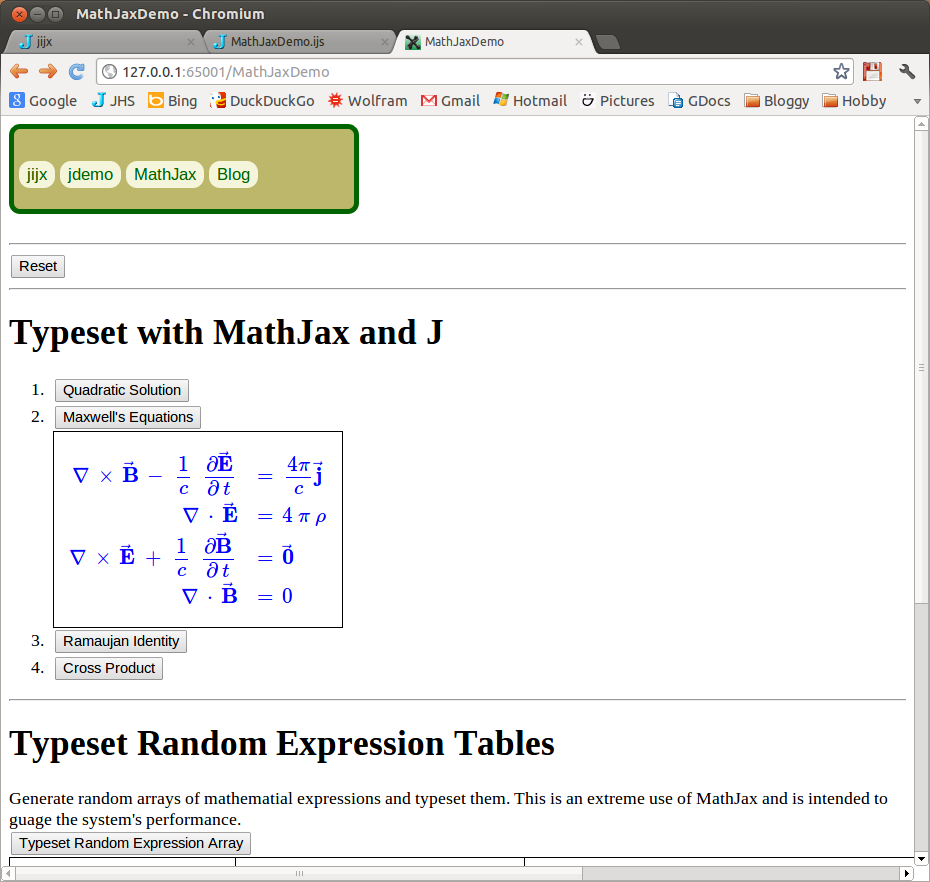
\includegraphics{mathjaxdemo.png}}
%Screen shot of JHS MathJaxDemo running on Ubuntu.
%{[}/caption{]}



%\captionsetup[floatingfigure]{labelformat=empty}
%\begin{figure}[htbp]
%\begin{floatingfigure}[l]{0.25\textwidth}
%\centering
%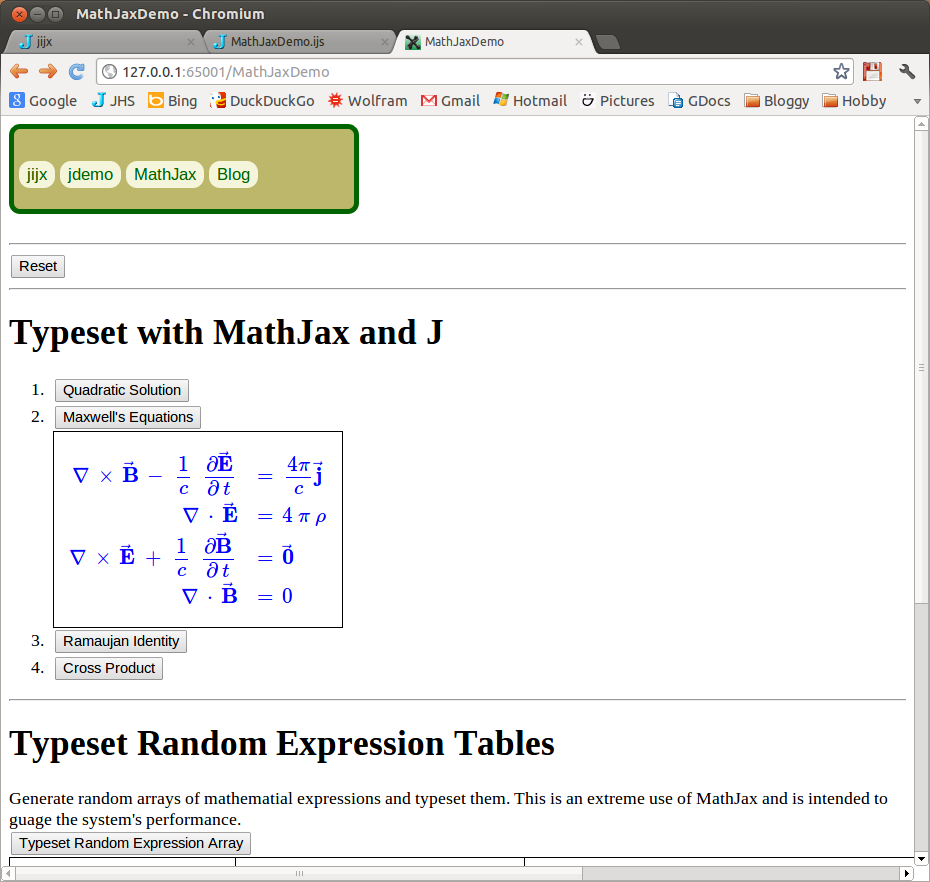
\includegraphics[width=0.23\textwidth]{mathjaxdemo.png}
%\caption{~~~IMCAPTION~~~}
%\label{fig:3402X0}
%\end{floatingfigure}
%\end{figure}



%\end{document}